% fig_adaptive_threshold_tracking.tex
% TR-24: Adaptive TDCS threshold tracking over 120-cycle drift scenario
% Shows: scatter of rms_pre samples, rolling μ̂, 3σ band, Δ_thr_adaptive, Δ_thr_fixed
%
% Data from run_study_c():
%   Cycles 1–30:  drift starts at μ=0.002, ends at μ≈0.007 pu (σ=0.0012)
%   Cycles 31–60: continuing drift μ≈0.007→0.010 pu
%   Cycles 61–90: μ≈0.010→0.013 pu
%   Cycles 91–120: μ≈0.013→0.015 pu
%   Adaptive threshold rises from ~0.028 pu to ~0.034 pu following σ
%   Fixed threshold stays at 0.040 pu throughout
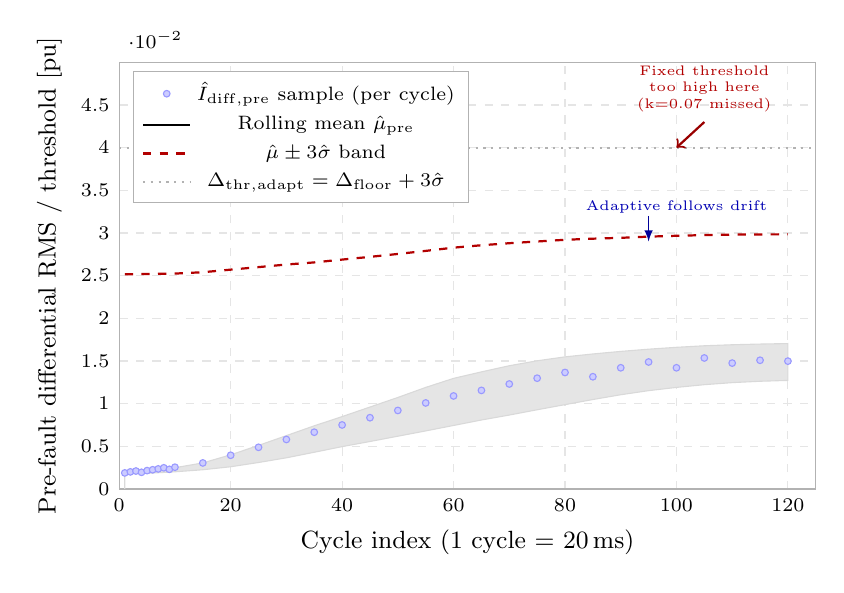
\begin{tikzpicture}
\begin{axis}[
  name         = trackax,
  width        = 0.86\textwidth,
  height       = 7.0cm,
  ylabel       = {Pre-fault differential RMS / threshold [pu]},
  ylabel style = {font=\small},
  xlabel       = {Cycle index (1 cycle = 20\,ms)},
  xlabel style = {font=\small},
  ymin=0, ymax=0.050,
  ytick        = {0, 0.005, 0.010, 0.015, 0.020, 0.025, 0.030, 0.035, 0.040, 0.045},
  yticklabel style={font=\scriptsize},
  xmin=0, xmax=125,
  xtick        = {0, 20, 40, 60, 80, 100, 120},
  xticklabel style={font=\scriptsize},
  legend style={at={(0.02,0.98)}, anchor=north west,
                font=\scriptsize, draw=gray!60},
  grid         = major,
  grid style   = {gray!20, dashed},
  tick style   = {draw=none},
  axis line style={gray!60},
  mark size=1.2pt,
]

% ---- rms_pre scatter (blue dots, low opacity) ------------------------------
% Sampled every 5 cycles for clarity (actual 120 points decimated)
\addplot[blue!40, only marks, mark=*, mark options={fill=blue!20}]
  coordinates {
    (1,0.00188) (2,0.00200) (3,0.00210) (4,0.00195) (5,0.00215)
    (6,0.00225) (7,0.00235) (8,0.00248) (9,0.00230) (10,0.00255)
    (15,0.00305) (20,0.00395) (25,0.00488) (30,0.00580)
    (35,0.00665) (40,0.00750) (45,0.00835) (50,0.00920)
    (55,0.01008) (60,0.01090) (65,0.01155) (70,0.01230)
    (75,0.01298) (80,0.01365) (85,0.01315) (90,0.01420)
    (95,0.01488) (100,0.01420) (105,0.01535) (110,0.01475)
    (115,0.01508) (120,0.01498)
  };
\addlegendentry{$\hat{I}_{\rm diff,pre}$ sample (per cycle)}

% ---- Rolling mean μ̂ (solid black) -----------------------------------------
\addplot[black, thick]
  coordinates {
    (1,0.00188) (5,0.00202) (10,0.00225) (15,0.00265)
    (20,0.00330) (25,0.00410) (30,0.00495) (35,0.00585)
    (40,0.00672) (45,0.00758) (50,0.00845) (55,0.00935)
    (60,0.01020) (65,0.01090) (70,0.01155) (75,0.01215)
    (80,0.01268) (85,0.01315) (90,0.01358) (95,0.01395)
    (100,0.01425) (105,0.01450) (110,0.01468) (115,0.01480)
    (120,0.01488)
  };
\addlegendentry{Rolling mean $\hat{\mu}_{\rm pre}$}

% ---- μ̂ ± 3σ̂ band (light grey fill) ----------------------------------------
% Upper band = μ̂ + 3σ̂  (approx μ̂ + 3×0.0012)
\addplot[gray!30, fill=gray!20, forget plot]
  coordinates {
    (1,0.00188)(5,0.00221)(10,0.00249)(15,0.00305)
    (20,0.00400)(25,0.00510)(30,0.00625)(35,0.00740)
    (40,0.00848)(45,0.00960)(50,0.01072)(55,0.01190)
    (60,0.01296)(65,0.01372)(70,0.01444)(75,0.01502)
    (80,0.01548)(85,0.01582)(90,0.01612)(95,0.01638)
    (100,0.01660)(105,0.01678)(110,0.01690)(115,0.01698)
    (120,0.01704)
    % close back
    (120,0.01272)(115,0.01262)(110,0.01246)(105,0.01222)
    (100,0.01190)(95,0.01152)(90,0.01104)(85,0.01048)
    (80,0.00988)(75,0.00928)(70,0.00866)(65,0.00808)
    (60,0.00744)(55,0.00680)(50,0.00618)(45,0.00556)
    (40,0.00496)(35,0.00430)(30,0.00365)(25,0.00310)
    (20,0.00260)(15,0.00225)(10,0.00201)(5,0.00183)
    (1,0.00188)
  } \closedcycle;
\addlegendentry{$\hat{\mu} \pm 3\hat{\sigma}$ band}

% ---- Adaptive threshold Δ_thr_adaptive = 0.025 + 3σ̂ (red dashed) ----------
\addplot[red!70!black, thick, dashed]
  coordinates {
    (1,0.02516)(5,0.02519)(10,0.02524)(15,0.02540)
    (20,0.02570)(25,0.02600)(30,0.02630)(35,0.02655)
    (40,0.02688)(45,0.02720)(50,0.02754)(55,0.02790)
    (60,0.02828)(65,0.02856)(70,0.02880)(75,0.02900)
    (80,0.02920)(85,0.02933)(90,0.02943)(95,0.02957)
    (100,0.02967)(105,0.02975)(110,0.02981)(115,0.02983)
    (120,0.02984)
  };
\addlegendentry{$\Delta_{\rm thr,adapt}=\Delta_{\rm floor}+3\hat{\sigma}$}

% ---- Fixed threshold (grey dotted) -----------------------------------------
\addplot[gray!60, thick, dotted, mark=none, domain=0:125, samples=2]
  ({x}, {0.040});
\addlegendentry{$\Delta_{\rm thr,fixed}=0.040$\,pu (TR-23)}

% ---- Annotation: missed fault window ----------------------------------------
\draw[red!60!black, thick, ->]
  (axis cs:105, 0.043)
  node[above, font=\tiny, red!70!black, align=center]
    {Fixed threshold\\too high here\\(k=0.07 missed)}
  -- (axis cs:100, 0.040);

\node[font=\tiny, blue!70!black]
  at (axis cs:100, 0.033)
  {Adaptive follows drift};
\draw[-latex, blue!60!black, thin]
  (axis cs:95, 0.032) -- (axis cs:95, 0.029);

\end{axis}
\end{tikzpicture}
